\documentclass[11pt]{iopart}
%Uncomment next line if AMS fonts required
%\usepackage{iopams}
\usepackage{graphicx}
\usepackage{siunitx}
\usepackage{textcomp}
\usepackage{booktabs}
\usepackage{caption} % to centre figure captions
\captionsetup{format=plain, font=small, labelfont=bf}
\usepackage[labelsep=period]{caption} % changes : to . in captions
%\captionsetup{labelfont=bf, labelsep=period}
\begin{document}

\title[Distances to Globular Clusters using RR Lyrae Variables]{Distances to Globular Clusters using RR Lyrae Variables}

\author{Luke Bischoff}

\address{Department of Physics, University of Bath, Bath BA2 7AY, United Kingdom}
\ead{ltb24@bath.ac.uk}
\begin{abstract}
RR Lyrae variable stars resident in two globular clusters in the Milky Way galaxy, Palomar 5 and Palomar 13, are analysed and the distances to the globular clusters determined. Point spread function photometry was performed on a series of observations taken from the Infrared Array Camera on board the \textit{Spitzer Space Telescope} in the mid-infrared bands, 3.6 $\mu$m (channel 1) and 4.5 $\mu$m (channel 2), to measure the apparent magnitudes of RR Lyrae stars detected with in the globular clusters. Apparent magnitudes were averaged using a Gaussian local estimation algorithm, which were then corrected for dust extinction effects. Period-luminosity relations were fit to the data for both clusters, from which distances in both the 3.6 $\mu$m and 4.5 $\mu$m bands were obtained. The average distance between each infrared band to the globular clusters were determined to be $d_{\rm Pal 5} = 20.37 \pm 0.51$ (random) $\pm 1.60$ (systematic) kpc, $d_{\rm Pal 13} = 24.25 \pm 0.62$ (random) $\pm 1.90$ (systematic) kpc which were found to be consistent with previous determinations.
\end{abstract}

\section{Introduction}

\subsection{The SMHASH program and Spitzer}
\label{smhash}
The measurement of distances to objects throughout the Universe is notoriously difficult due to the absence of direct three-dimensional information available and remains an active area for research in astrophysics. Observations made using the \textit{Spitzer Space Telescope} as part of the  \textit{Spitzer} Merger History and Shape of the Galactic Halo (SMHASH), alongside the Carnegie RR Lyrae Program (CRRP) can be used to measure distances in the local universe to a higher accuracy than before \cite{monson2017}. The SMHASH program primarily aims to construct a three-dimensional map of the Milky Way (MW) galaxy \cite{garofalo2018smhash} by using mid-infrared observations of RR Lyrae (RRL) variable stars in globular clusters and dwarf spheroidal galaxies (dSphs) of the MW. The CRRP, which is complementary to the SMHASH program, studies RRLs in the MW \cite{muraveva2018crrp} and so, together, these programs are contingent on accurate determinations of distances.

In this paper, distances to the Palomar 5 (Pal 5) and Palomar 13 (Pal 13) globular clusters are calculated using the Infrared Array Camera (IRAC) on board the \textit{Spitzer Space Telescope} as part of the Warm Mission during 2013, using its 3.6 $\mu$m and 4.5 $\mu$m channels; after \textit{Spitzer's} cryogenic coolant run out, thus ending the use of its two longer wavebands.

\subsection{RR Lyrae variables}
\label{rrls}
RR Lyrae stars are Population II variable stars, meaning they are relatively old and metal-poor stars that vary with regular periods of around a few hours to a day \cite{beaton2016}. RRLs are frequently found in large quantities with in globular clusters which reside in the galactic halo of the MW galaxy. Starting life on the main sequence with masses typically less than that of the Sun, RRLs have evolved past their red-giant stage to lie on the instability strip of the Hertzsprung-Russell diagram \cite{muraveva2020}. There are three main types of RRL: (i) RRab types which pulsate in the fundamental frequency, (ii) RRc types which pulsate in the first overtone, typically with smaller amplitudes but in a more sinusoidal fashion than RRab types, and, (iii) RRd types which pulsate simultaneously in the fundamental frequency and the first overtone \cite{monson2017}. Due to their regular variation in brightness, RRL stars are used as standard candles, which are markers used to calibrate distances to cosmological objects \cite{garofalo2018smhash}.

Previous work has typically focused on Cepheid variable stars and the Cepheid period-luminosity (PL) relation, known as the Leavitt law after being discovered by Henrietta Swan Leavitt in 1908. A PL relation is the relationship between a star's brightness and its period of pulsation. PL relations compare a variable star's Cepheids, like RRLs, are used as standard candles but are brighter and pulsate with a longer, more stable period of around weeks, when compared to RRLs \cite{beaton2016}. The PL relations of Cepheids are well defined in optical wavebands, however this leaves them susceptible to dust extinction effects \cite{scowcroft2011}. Therefore, RRL PL relations in the mid-infrared bands have several advantages over Cepheids, such as (i) weaker effects due to dust extinction, (ii) metallicity effects are damped in these wavebands, (iii) more sinusoidal and symmetrical light curves with smaller amplitudes improve precision of average apparent magnitudes, and (iv) a narrower dispersion (or scatter) in the PL relations \cite{garofalo2018smhash, beaton2016}. 

The cosmic distance ladder details a process of using cosmological objects, such as Cepheids and RRLs, to calibrate distances from the galactic neighbourhood of around 10 kpc up to 100 Mpc with an ultimate aim to accurate measure the Hubble constant, $H_{0}$. Initially Cepheids and the Leavitt law have been used to climb the distance ladder, however results for the Hubble constant remain inconsistent depending on the approach \cite{beaton2016}. Determinations of the Hubble constant using Cepheids have yielded values of $H_{0} = 74 \pm 3$ kms\textsuperscript{-1}Mpc\textsuperscript{-1} \cite{freedman2012hubble} where as determinations using the cosmic microwave background have obtained values of $H_{0} = 67.8 \pm 0.9$ kms\textsuperscript{-1}Mpc\textsuperscript{-1} \cite{planckcollab}. This inconsistency could be resolved by using RRLs as a separate route up the cosmic distance ladder which could improve the precision of the Hubble constant to less than 3\% \cite{beaton2016}. An agreement for a precise value of the Hubble constant would enable an appreciation of the age, size and expansion of the Universe \cite{freedman2001hubble} highlighting the importance of obtaining accurate measurements for these first rungs of the cosmic distance ladder.

\section{Data selection and photometry}
\label{dataselectionphot}

\subsection{Data selection}
\label{dataselection}

The IRAC on board \texit{Spitzer} observed a region of around 6$\times$15 arcminutes around the centres of the Pal 5 and Pal 13 globular clusters. Pal 5 \cite{erkal2017} and Pal 13 \cite{bradford2011} both exhibit long tidal streams that extend beyond their centres due to interaction with, and accretion to, the MW galaxy, and so RRLs residing within these tidal streams are not observed. Each cluster was observed in both the 3.6 $\mu$m (IRAC channel 1) and 4.5 $\mu$m (IRAC channel 2) wavebands and over a duration of 12 epochs, with one frame in each channel per epoch, calibrated such that at least one full cycle for each RRL in the frame was observed. Prior to use, the raw data was pre-processed into basic calibrated data (BCD) frames by \texit{Spitzer} Science Centre using an established pipeline to reduce the images into a useable state. Image reduction, for example, involves flat fielding of the images, which is a corrects for variations in pixel sentivity across the detector and the removal of biases \cite{reach2005absolute}. Mosaic frames, which is a stitching together of individual BCDs, for each epoch in both IRAC channels were created by the supervisor for this project, Dr Victoria Scowcroft, resulting in the final data in the form of Flexible Image Transport System (\verb"FITS") files. A pixel phase effect can be exhibited on individual BCDs due to differences in flux depending on the location within a pixel the light from a point sources falls because of quantum efficiency variations \cite{irachandbook}, however because the combination of the BCDs into mosaics smooths out this pixel phase effect, correction for it was neglected.

The positions in right ascension (RA) and declination (Dec), periods in days and the type of previously known RRLs were obtained from the \textit{Catalogue of Variable Stars in Galactic Globular Clusters} (CVS), maintained by Christine Clement \cite{clement}. Further information was gathered from \textit{Gaia} Data Release 2 (\textit{Gaia} DR2) \cite{gaia} by considering a region of 10' in radius around the centre of the globular clusters and searching for stars marked as \verb"variable". The variable stars identified were checked against the RRLs in the CVS to identify candidate RRLs missing from the CVS. Confirmation of whether the candidate variable stars from the region search in \textit{Gaia} was obtained by matching the \textit{Gaia} \verb"source_id" of the candidate stars to the \verb"gaiadr2.vari_rrlyrae" list containing information on 140784 RRLs; including their periods and types. If the period of the RRL was available from \textit{Gaia}, then this was used over the periods provided in the CVS because some periods in the CVS were obtained in 1962 \cite{kinman1962notes} and RRL periods are not necessarily stable over human lifetimes (ref).

Master mosaic images were also created for each IRAC channel to create \verb"FITS" files of a median image using data from across all 12 epochs. By creating a median image, the master mosaic images have a higher signal-to-noise ratio, making them particularly useful as a comparison to the individual epoch data. The data for the SMHASH program and CRRP were optimised for IRAC channel 1 in the 3.6 $\mu$m band and so the channel 2 data, taken in the 4.5 $\mu$m band, has a lower signal-to-noise ration which presented some issues, particularly regarding the individual epoch data, which is explained more in section \ref{light curves} \cite{garofalo2018smhash}.

The individual \verb"FITS" files, as well as the image data as flux values in MJysr\textsuperscript{-1},  contained header information detailing the exposure time, observation date and time and a flux conversion factor for both the epoch files and the master moasic files. This information was used to convert the flux values from MJysr\textsuperscript{-1} into data number counts, DN, using Equation 1,
\begin{equation}
\label{eq:conv}
    counts\;=flux\;\cdot \frac{exposure\;time}{flux\;conversion\;factor}\;.
\end{equation}
where flux is in MJysr\textsuperscript{-1}, exposure time is in seconds and the flux conversion factor in MJysr\textsuperscript{-1}$\cdot$ DN\textsuperscript{-1}$\cdot$ s.

\subsection{Photometry}
\label{photometry}

Photometry involves measuring the amount of light, usually in flux or data number counts, from the image produced by a detector or camera, such as IRAC \cite{ccdastron}. Once the epoch and master mosaic data was converted into DN counts, photometry was performed on the data to obtain the apparent magnitudes of point sources detected in the frames. There are two main methods for performing photometry that were considered during this project, aperture photometry and point spread function (PSF) photometry. Aperture photometry involves considering the flux of light measured through an aperture centred on the star of radius just larger than the star. A second aperture of larger radius than the aforementioned aperture is also drawn and centred to form an annulus around the star. The average background flux measured in the annulus region is then subtracted from the inner aperture to obtain the flux of the star. There is a problem of optimisation here, particularly regarding the radii of the inner and outer apertures, as such it is necessary to ensure that an aperture is chosen that is not too large to include contamination by nearby sources of light but also not too small such that light from the star is being omitted and counted as background flux (CLARIFY). 

The second method, PSF photometry, involves building a model based on the images of point sources that are detected and typical of a particular detector and fitting the model to point sources in the image frames in order to measure the flux of each point source \cite{ccdastron}. The process is usually iterative in that the stars that have been fit and flux values measured are subtracted from the image to create a residual image. The process of fitting the model to the residual image is then completed which may reveal stars that were not detected in the previous iteration. This iterative process applied by PSF photometry is particularly useful for crowded fields and because globular clusters are crowded in nature, PSF photometry was chosen over aperture photometry.

\subsubsection{PSF model.}
A point spread function can be thought of as the image profile produced by a particular instrument, such as IRAC, when a point source is incident on it. The idea of an \textit{effective} PSF (ePSF) model is introduced in Anderson and King \cite{andersonking2000}, which is a net PSF describing the amount of light from a point source falling on an individual pixel. Separate ePSF models were built from the master mosaic frames for each IRAC channel because the model is dependent on the sample of stars present in each frame. This ensures that an accurate ePSF model is produced to reduce the number of false positive and false negative detections of point sources, when the model is eventually fit to the series of epoch frames. Individual epoch frames were at first used to develop ePSF models to be used in the photometry of that corresponding epoch, however, some epoch frames had particularly low signal-to-noise ratios; especially in channel 2. This meant that inaccurate or failed ePSF models were built, resulting in defects in the PSF photometry process causing inaccurate apparent magnitudes. Therefore, the master frames were used to develop ePSF models, which, as a result of their higher signal-to-noise ratio, improved the quality of the model.

Stars used to construct the ePSF models were detected using a point source detection algorithm, \verb"DAOStarFinder", which implements the \verb"DAOFIND" routine of the greater \verb"DAOPHOT" procedure, developed by Peter Stetson \cite{stetson1987}. A version of the \verb"DAOPHOT" procedure is usefully included in the Python package, \verb"photutils" \cite{photutils}, which was used extensively throughout this project. Bright stars, above a threshold of 50$\sigma$ from the background level, were chosen for the ePSF model because these stars are more well-defined, with a higher signal-to-noise ratio, to ensure an accurate ePSF model was derived for each IRAC channel. Stars residing near the edge of the master mosaic frames were discounted from the detections and each candidate star to be used in the ePSF model was presented in a list of images and manually inspected for defects. Candidate stars exhibiting defects such as a blending effect, which could be two or more unresolved stars or a galaxy; crowding from neighbouring stars or stars containing artefacts such as bad pixels or cosmic rays. Detection parameters were utilised, which were implemented as part of the source detection algorithm (see section 2.2.2), which greatly reduced detections of candidate stars containing these artefacts, however, the candidate stars were still screened for these defects as some artefacts were still detected. Once these poor quality candidate stars were removed from the list, the ePSF model was rebuilt and saved ready for use in the photometry routine.

\subsubsection{PSF photometry.}
A master source list containing all detected point sources was generated from the master mosaic frame for each IRAC channel in both globular clusters. The star detection algorithm was run on the frames as part of the PSF routine based on each channel's respective ePSF model to populate the master source list to which can be referred to when performing photometry on the series of epoch frames.

Several parameters for the source detection algorithm were used to reduce the number of false positive star detections, these are the full width at half maximum (FWHM) of the stars, a threshold detection value and two parameters relating to the shape and sharpness of the point sources. The optimisation problem must be reconsidered again when deciding on the specific values to use in order to select values which are sufficient enough to ensure actual stars are detected but not to such a degree that, for example, random noise is being detected as a star or that the process becomes computationally time expensive. The FWHM parameter was determined based upon analysis of the radial profiles of many uncrowded stars in the frames. The radial profiles of these stars were manually examined using \verb"ImExam", an affiliated package of the Python package, \verb"astropy", as in table 1 of The Astropy Collaboration \textit{et al} \cite{astropy}. After gaining an appreciation for the range of FWHM values, a value of 5.0 pixels was deemed acceptable.

The second parameter considered is the threshold value, measured in standard deviations, $\sigma$, above the median background level. Only point sources with peak count values above the determined threshold value will be detected as a star. A plot of the number of sources detected vs threshold value was generated with a range of threshold values from 1$\sigma$ to 10$\sigma$, producing an "elbowed" curve, where the elbow of the curve was situated around 5$\sigma$ to 6$\sigma$. A value of 50$\sigma$ was used in building the ePSF models, but this was a special case as explained in section 2.2.1. Instead, for the source detection algorithm on the master and epoch frames, a value of 6$\sigma$ was decided for the threshold value after considering the location of the elbow on the $x$-axis of aforementioned plot.

Another parameter that was analysed was the \verb"round" parameter, which considers the profiles of the point sources and aims to discard sources with directional biases, which could indicate that the source is a galaxy, for example, instead of a star. After visual examination of detected sources, values of $\pm$0.5 were used. The \verb"sharp" parameter is the final parameter examined here, which considers the sharpness of the profile of the point sources and so setting an upper limit on the sharpness aims to avoid the source detection algorithm detecting bad pixels or cosmic rays as stars. This value, also determined by visual examination, was set to an upper limit of 0.8 for the construction of the ePSF models, because the most accurate model was desired; the value was relaxed to 0.9 for detections in the master and epoch frames.

Photometry was then performed using an iteratively subtracted PSF routine, which follows the process outlined in \verb"DAOPHOT" \cite{stetson1987}, whereby the source detection algorithm is run in accordance with the parameters described previously, to measure the flux, in DN counts, of the sources in the epoch frames. The ePSF model constructed for each channel is fit to the epoch data using the Levenberg-Marquardt algorithm and least squares statistic built into \verb"astropy" \cite{astropy}. A fixed centroids process, which reduces the uncertainty in the determinations of flux \cite{garofalo2018smhash}, was undertaken by using the initial positions of sources in the master source list, to improve the precision of the detected sources within the PSF photometry routine. A residual image was obtained after the fitted sources were subtracted from the image, ready for the next iteration of the process. Pal 5 and Pal 13 are relatively uncrowded compared to other globular clusters and so only 2 iterations was needed. Once the iterative process was completed, values for the magntidues of detected stars in DN were obtained for that epoch.

The process was slightly modified for IRAC channel 2 of Pal 13, such that the PSF photometry only considered regions of 50$\times$50 pixels around known RRLs using the CVS and \textit{Gaia} data due to an extremely bright source in the frame which resulted in no values for magnitudes of sources in most epochs being obtained. The rest of the analysis was the same as in the previous paragraph, only the initial sources stage was changed.

The coordinates of stars detected in the epoch frames were converted from their $x$ and $y$ values into RA and Dec using the given World Coordinate System (WCS) \cite{astropy} in the header of the \verb"FITS" files and transformed using the International Celestial Reference System (ICRS). This was necessary because the $x$ and $y$ coordinates of the stars in each epoch frame are unique to that frame only and so coordinates common to all epoch frames (including the master frame) were required to enable identification of the same sources in each frame. The PSF photometry routine was completed on all 12 epochs in series, for both channels, each time matching the stars detected in the epoch to the master frame using the WCS transformations. A final list of sources containing their positions in RA and Dec, their magnitudes in DN and uncertainties in DN for each epoch was obtained.

\subsection{Determination of apparent magnitudes}

The apparent magnitude, $m$, of each star was calculated using Equation 2,
\begin{equation}
\label{eq:mag}
    m = ZP - 2.5\log_{10} \left(counts \cdot \frac{flux\;conv \cdot aperture\;correction \cdot loc\;correction}{exposure\;time}\right),
\end{equation}
where $ZP$ is the zero-point magnitude for each IRAC channel, which is 18.80 for channel 1 and 18.32 for channel 2 as per the IRAC Handbook \cite{irachandbook}, $counts$ is the flux in DN obtained from the photometry, the flux conversion factor and exposure time used to convert $counts$ back into flux values. An aperture correction has also been applied to account for the difference between the apertures used to calibrate IRAC and the aperture of 6 pixels used to perform the photometry. The $loc\;correction$ in Equation 2 is an array-location dependent correction which is a \verb"FITS" file that corrects for scattering and spatial distortion caused by IRAC \cite{irachandbook}. The uncertainty in magnitudes was also calculated during the PSF photometry routine and was propagated through into magnitudes. The uncertainties in apparent magnitude primarily arise due to the fitting process of the ePSF model, for example, it's finite accuracy and errors in the fit caused by blending or contamination from nearby stars \cite{stetson1987}.

\subsection{Light curves}
\label{light curves}
Light curves are plotted to identify and examine how the brightness of the stars vary as a function of time or, as in Figure 1, phase. An assortment of light curves are shown in Figure 1 from both Pal 5 and Pal 13 to give some examples of light curves from the data analysed and show some variations between them.

The phase of the light curves was obtained by first extracting the date and time each epoch frame was taken from the header of the \verb"FITS" file and converting this into a Modified Julian Date (MJD). From there, the phase was calculated using Equation 3,
\begin{equation}
    \phi = \frac{[MJD]}{P} - \left\lfloor\frac{[MJD]}{P}\right\rfloor,
\end{equation}
where $[MJD]$ is the time in Modified Julian Date and $P$ is the period of the RRL, similar to equation 10 in Monson \textit{et al} \cite{monson2017}. The phase has been calculated so that multiple periods of the RRLs can be displayed in the light curve because only one period worth of raw data was collected, and so phase is a useful way to check whether the periods smoothly join together.
\begin{figure}
    \centering
    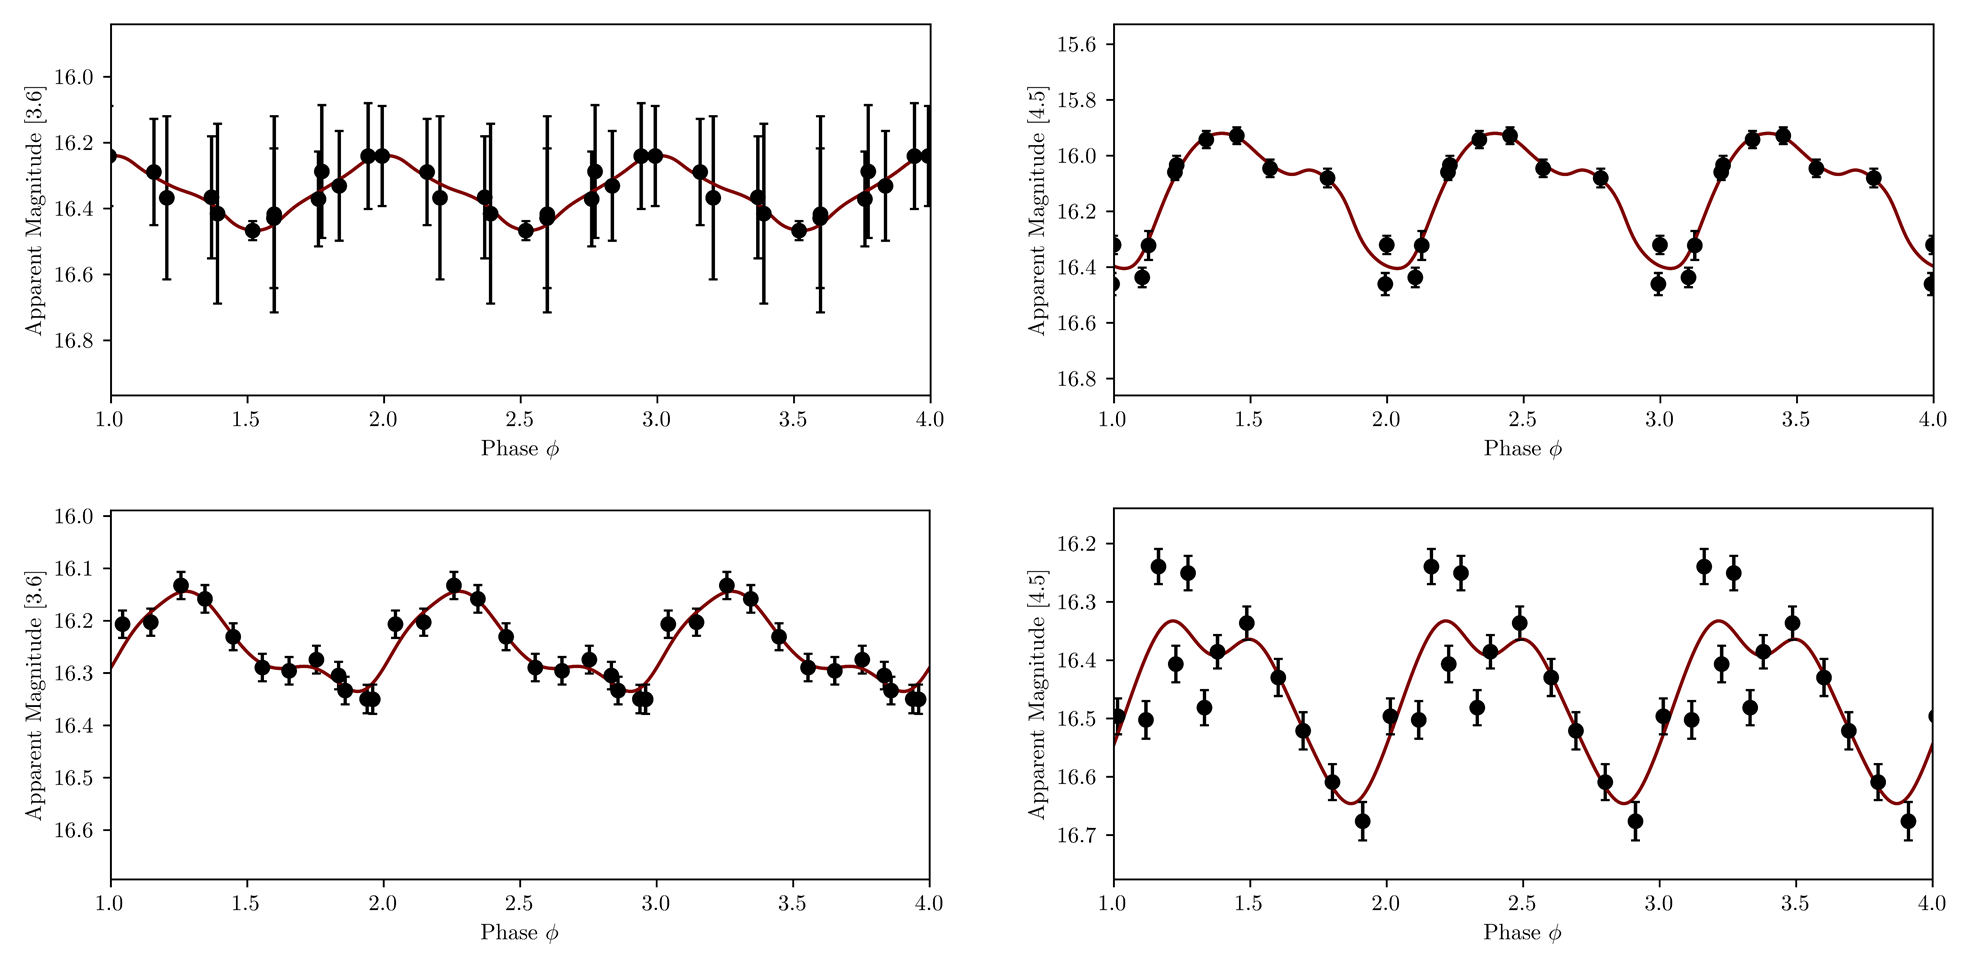
\includegraphics[scale=0.3]{all_lcs.png} % original scale 0.55 for old img
    \footnotesize
    \caption{A summary of light curves from Pal 5 (top) and Pal 13 (bottom), displaying the range of curves obtained for the two globular clusters. a) the channel 1 light curve for RRL1, an RRc star in Pal 5 exhibiting large uncertainties in apparent magnitude. b) the channel 2 light curve of RRL7, an RRab star in Pal 5. c) the channel 1 light curve for RR1, an RRab star of Pal 13 displaying a characteristic curve of RRab type stars with minimal defects. d) the channel 2 light curve for RRL4, an RRab star in Pal 13 exhibiting scatter about the GLOESS fit.}
    \label{fig:light curves}
    \normalsize
\end{figure}
A Gaussian local estimation algorithm (GLOESS) \cite{persson2004} has been used to fit a curve to the light curves and to calculate the time-averaged apparent magnitudes and corresponding uncertainties of the RRLs by parsing the algorithm the phase, apparent magnitude and magnitude uncertainties of each RRL. GLOESS uses second-order polynomials to fit the data locally via interpolation between subsequent data points on the $x$ axis \cite{monson2012} and moves across the data set until the entire light curve has been processed. This time-averaged (mean) apparent magnitude for each RRL was extracted and placed into an array containing its corresponding uncertainty and period. The uncertainty in the mean apparent magnitude was calculated using Equation 4,
\begin{equation}
    \sigma_{\langle m\rangle} = \sqrt{\frac{\Sigma \sigma_i^2}{N^2} + \sigma_{\rm fit}^2 + A^2}\:,
\end{equation}
where $\sigma_i^2$ is the uncertainty in each individual epoch's apparent magnitude for that RRL, $N$ is the number of epochs present in the light curve, $\sigma_{\rm fit}^2$ is the standard deviation of the points around the fit and $A$ is the value of the dust extinction.

The average apparent magnitudes were corrected for extinction effects caused by dust in the MW galaxy between the observer and the globular cluster. This results in a reddening of the apparent magnitudes which would influence the measured distances to the globular clusters. The corrections for dust extinction were obtained from the IRSA Dust Extinction Service Queries built into the \verb"astroquery" module in Python \cite{Ginsburg2019}, which uses a MW dust map developed in 2011 \cite{schlafly2011measuring}. Extinction magnitudes, $A$, were subtracted from the mean apparent magnitudes for all of the RRLs detected. The extinction magnitudes were found to be only 0.1\% of the general sample's mean apparent magnitudes and with the absence of uncertainty values provided for the extinction corrections, the extinction value itself was taken as its uncertainty in Equation 4, which is consistent with, for example, Scowcroft \textit{et al} \cite{scowcroft2011}.

\section{Period-Luminosity relations and distance measurements}
\label{pl and distances}
\subsection{Fitting PL relations for Pal 5 and Pal 13}
In order to calculate the distance to the globular clusters, a comparison between the apparent magnitude of the RRLs and their absolute magnitudes is required. This can be done by comparing a calibrated PL relation from the literature to a PL relation fit, by using the same mathematical form as the calibrated PL relation, to the sample data. The PL relations that have been fit to the data in Figures 2 and 3, for Pal 5 and Pal 13 respectively, use the PL relation data provided in table 3 of Neeley \textit{et al.} \cite{neeley2019} (henceforth N19), which is the most recent set of PL relations covering both IRAC channels 1 and 2.

The calibrated PL relations, for both apparent magnitude and absolute magnitude take the form of Equation 5,
\begin{equation}
    M = a + b\left(\log_{10}(P) + 0.3\right)\,,
\end{equation}
where $M$ is the apparent or absolute magnitude, $a$ is the $y$-intercept of the PL fit, $b$ is the gradient of the PL fit and $P$ is the period of the RRL.

Prior to fitting the PL relations, RRLs identified as type RRc stars, were fundamentalised to enable comparisons between the RRc and RRab stars \cite{iben1974post}, using Equation 6,
\begin{equation}
    \log_{10}(P) = \log_{10}(P_{\rm FO}) + 0.127\,,
\end{equation}
where $P$ is the fundamentalised period and $P_{\rm FO}$ is the first overtone period. The exact form of the calibrated PL relations in absolute magnitudes are shown as Equation 7,
\begin{equation}
\label{eq:PL}
    \eqalign{M_{[3.6]} = -0.40(\pm 0.03) -2.78(\pm 0.38) (\log_{10}(P + 0.3))\,,\\
    M_{[4.5]} = -0.41(\pm 0.03) -2.83(\pm 0.39) (\log_{10}(P + 0.3))\,,}
\end{equation}
where the coefficients of $a$ and $b$ from Equation 5 are given in table 3 of N19. The PL relations in Figures 2 and 3 have been fit by fixing the gradient $b$ constant, while allowing $a$ to vary. Therefore, the PL relations shown in Figures 2 and 3, are of the form,
\begin{equation}
\label{eq:PL}
    \eqalign{m_{[3.6]} = a_{0} -2.78(\pm 0.38) (\log_{10}(P + 0.3))\,,\\
    m_{[4.5]} = a_{0} -2.83(\pm 0.39) (\log_{10}(P + 0.3))\,,}
\end{equation}
where $m$ is the average apparent magnitude and $a_{0}$ is the $y$-intercept, yet to be found.

\begin{table}
\caption{\label{table:results}Summary of the results and uncertainties for the apparent magnitude $m$ (as the intercept of the PL relation), distance modulus $\mu$ and distance $d$ obtained for Pal 5 and Pal 13.}
\footnotesize
\centering
\begin{tabular}{ccccccccccc}
\br
      &     & Pal 5 &       &      & Pal 13  &       \\
        \cmidrule(lr){2-4}\cmidrule(lr){5-7}
IRAC          & $m$  & $\mu$   & $d$    & $m$ & $\mu$  & $d$   \\
Channel      & (mag) & (mag) & (kpc) & (mag) & (mag) & (kpc) \\
          \mr
{[}3.6{]} & $16.10 & 16.51 & 20.04 & 16.47  & 16.88 & 23.80$ \\
\pm \sigma_{\rm rand} (\pm \sigma_{\rm sys})   & $\pm0.03 & \pm0.04 (\pm0.12) & \pm0.37 (\pm1.11) & \pm0.01  & \pm0.03 (\pm0.12) & \pm0.38 (\pm1.32)$ \\
             \mr
{[}4.5{]} & $16.16 & 16.57 & 20.69 & 16.55  & 16.96 & 24.69$ \\
\pm \sigma_{\rm rand} (\pm \sigma_{\rm sys})   & $\pm0.02 & \pm0.04 (\pm0.12) & \pm0.35 (\pm1.15) & \pm0.01  & \pm0.03 (\pm0.12) & \pm0.49 (\pm1.37)$ \\
\br
\end{tabular}
\normalsize
\end{table}
\begin{figure}
    \centering
    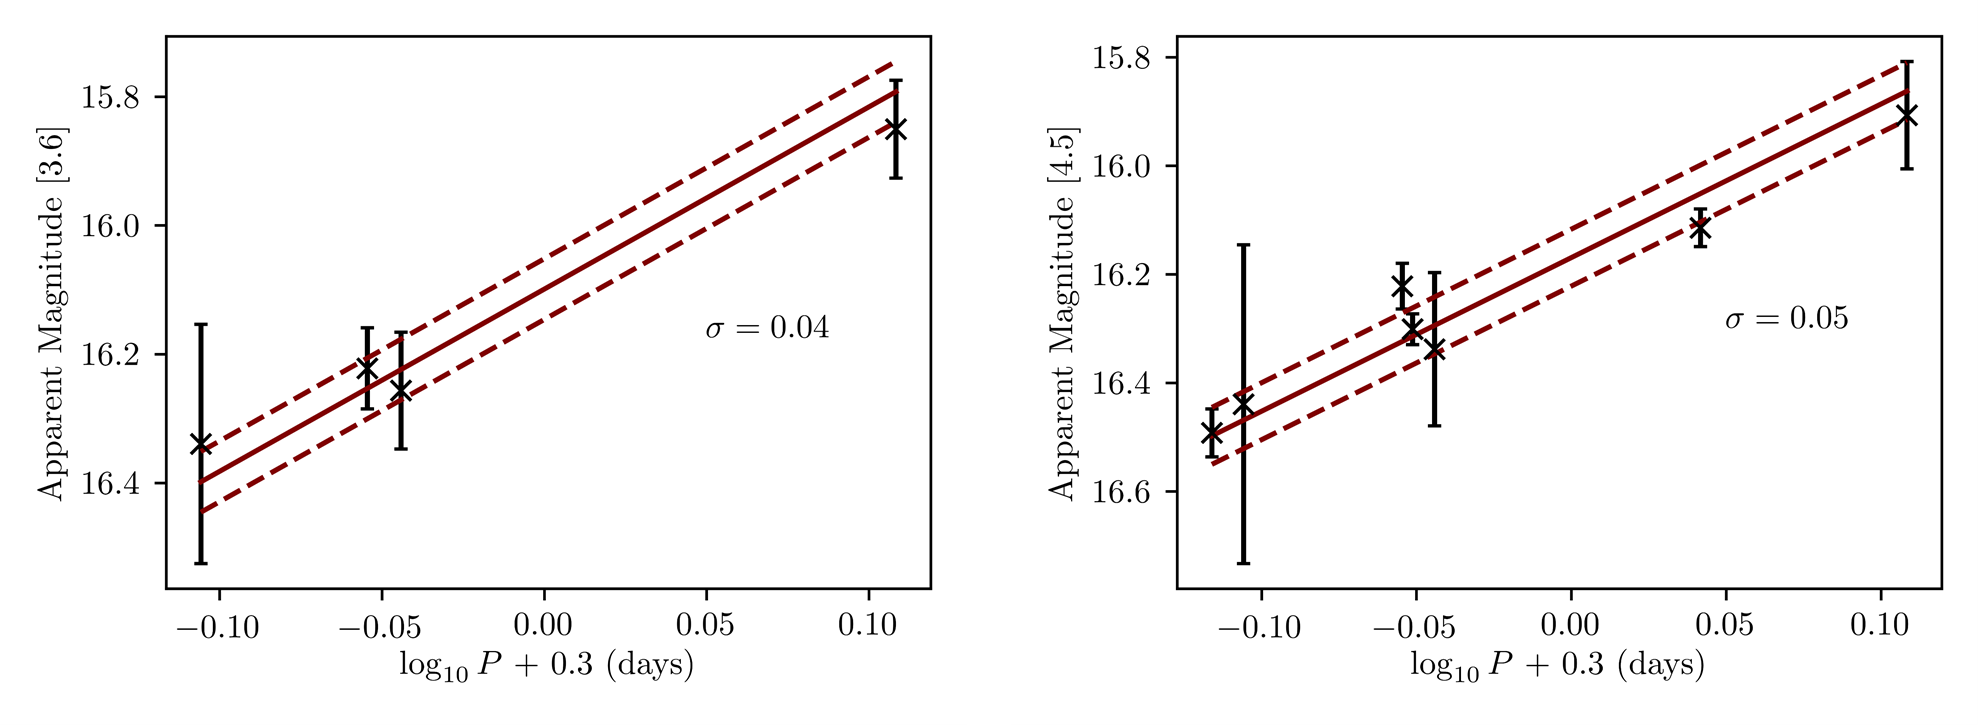
\includegraphics[width=\textwidth]{pal5_pl_test2.png}
    \footnotesize
    \caption{PL relations in channel 1 (left) and channel 2 (right) for Pal 5. The dashed lines indicate dispersion about the fitted PL, with the region between them being $\pm1\sigma$ of the residuals of the data points, as quoted for each PL relation. The periods of RRc and RRd stars have been fundamentalised in these PL relations.}
    \label{fig:PL}
    \normalsize
\end{figure}
\begin{figure}
    \centering
    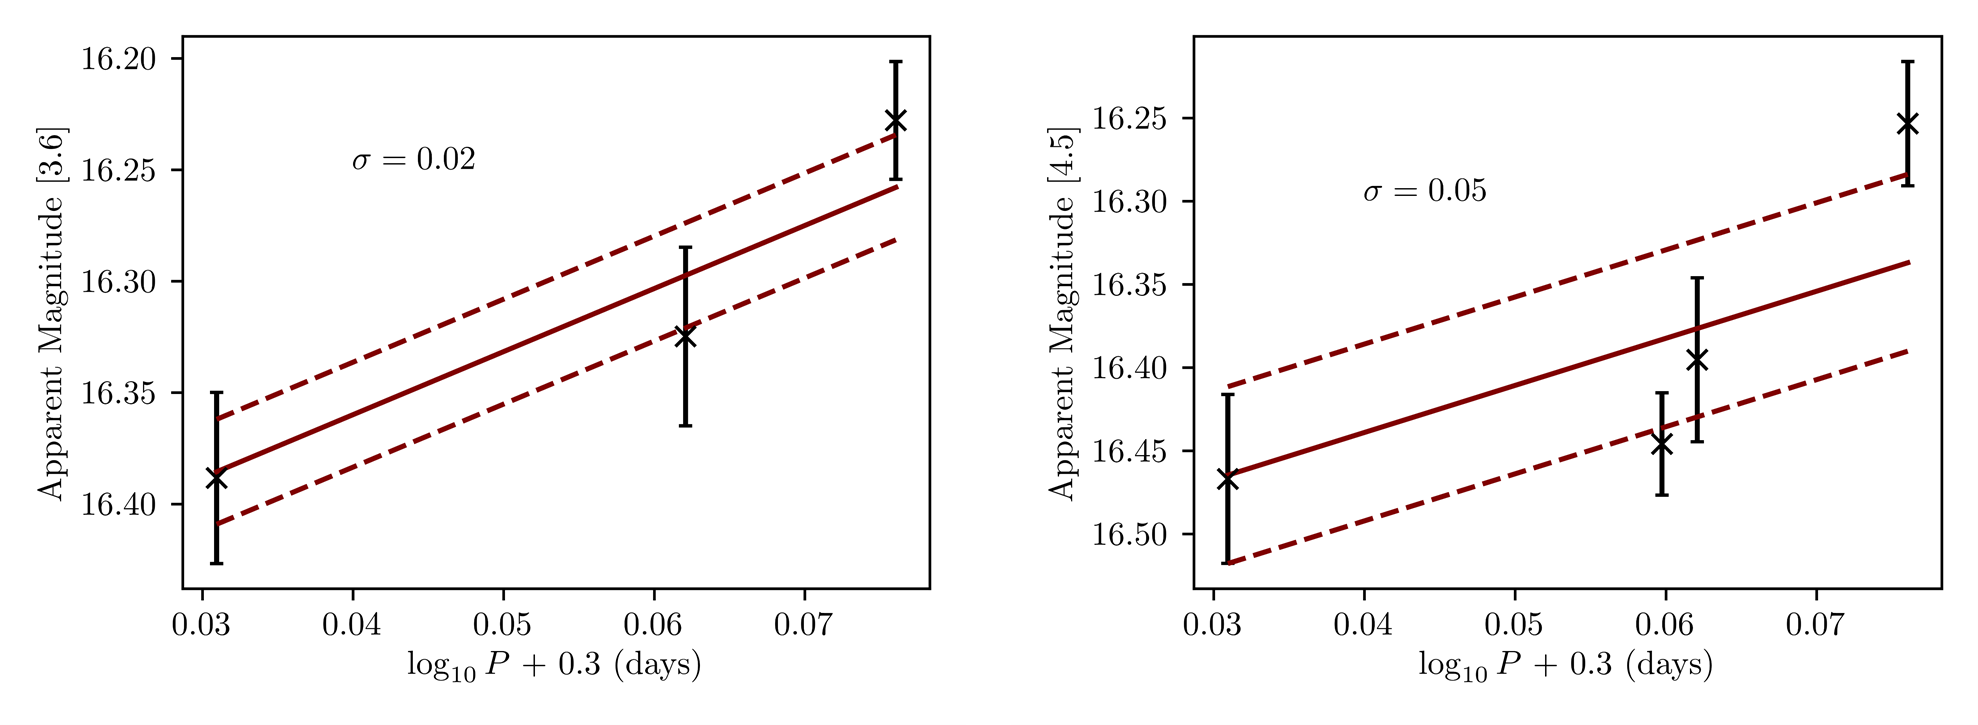
\includegraphics[width=\textwidth]{pal13_pl.png}
    \footnotesize
    \caption{PL relations in channel 1 (left) and channel 2 (right) for Pal 13. The dashed lines indicate dispersion about the fitted PL, with the region between them being $\pm1\sigma$ of the residuals of the data points, as quoted for each PL relation. There were no RRc or RRd stars in this sample of RRLs and so all RRLs in these PL relations are of type RRab.}
    \label{fig:PL}
    \normalsize
\end{figure}

The intercepts were found using a least-squares fit to obtain intercept values in both channels for Pal 5 as $a_{0[3.6]} = 16.10\pm0.03$ mag and $a_{0[4.5]} = 16.16\pm0.03$ mag; and in both channels for Pal 13 as $a_{0[3.6]} = 16.47\pm0.02$ mag and $a_{0[4.5]} = 16.55\pm0.03$ mag. The dispersion lines in Figures 2 and 3 represent one standard deviation $(\pm1\sigma)$ of the residuals of the RRL data points above and below the fitted PL relations; with a value quoted for each PL relation.



\subsection{Calculating distances to Pal 5 and Pal 13}
The distance to a globular cluster can be calculated from the distance modulus, which is the difference between the apparent magnitude and the absolute magnitude,
\begin{equation}
    \mu = m - M,
\end{equation}
where $\mu$ is the distance modulus, $m$ is the apparent magnitude and $M$ is the absolute magnitude. Consider the PL relations in Equations 7 and 8, the distance modulus for each IRAC channel can be found by subtracting Equation 7 from Equation 8, giving a general distance modulus,
\begin{equation}
    \mu = m - M = a_{0} - a,
\end{equation}
where $a_{0}$ is the calculated intercept from fitting the PL relations and $a$ is the intercept given in N19. The distance modulus for each channel can be obtained by substituting the relevant data for each IRAC channel into Equation 10. Therefore, the distance moduli values in both IRAC channels for Pal 5 are $\mu_{[3.6]} = 16.51\pm0.04$ $(\pm0.12)$ mag and $\mu_{[4.5]} = 16.57\pm0.04$ $(\pm0.12)$ mag and for Pal 13 are $\mu_{[3.6]} = 16.88\pm0.04$ $(\pm0.12)$ mag and $\mu_{[4.5]} = 16.96\pm0.04$ $(\pm0.12)$ mag. The first uncertainty quoted in the distance modulus results is the random uncertainty given by, $\sigma_{\rm rand} = \sqrt{\sigma_{a}^2 + \sigma_{a_{0}}^2}$, where $\sigma_{a}$ is the uncertainty in the calibrated intercept from N19 and in Equation 7 and $\sigma_{a_{0}}$ is the uncertainty in the calculated intercept as a result of the fitting process. The uncertainty quoted in brackets is the systematic uncertainty, which is the uncertainty in the PL relation itself and given by, $ \sigma_{\rm sys} = \sqrt{\sigma_{a}^2 + (0.3\cdot\sigma_{b}^2)}$, where $\sigma_{b}$ is the uncertainty in the gradient of the PL relation as given in N19 and Equation 7.

The distance, $d$, in parsecs (pc) can be calculated from the distance modulus by,
\begin{equation}
    \mu = 5\cdot\log_{10}(d) - 5,
\end{equation}
which can be rearranged for $d$, as shown in Equation 12,
\begin{equation}
    d = 10^{\frac{\mu}{5} + 1}.
\end{equation}
Therefore, the determined distances in both IRAC channels to Pal 5 (in kpc) are $d_{[3.6]} = 20.04\pm0.37$ $(\pm1.11)$ kpc and $d_{[4.5]} = 20.69\pm0.35$ $(\pm1.15)$ and for Pal 13 are $d_{[3.6]} = 23.80\pm0.38$ $(\pm1.32)$ kpc and $d_{[4.5]} = 24.69\pm0.49$ $(\pm1.37)$ kpc, where the uncertainties have been propagated through to kpc. A summary of these results are presented in Table 1.

\section{Discussion}
\subsection{Comparing results to previous literature values}
The distances to Pal 5 in both IRAC channels in Table 1 are consistent with each other when the random and systematic uncertainties are considered and so a mean distance to Pal 5 is determined to be $d_{\rm Pal 5} = 20.37\pm0.51$ $(\pm1.60)$ kpc, where the uncertainty is calculated as the quadrature sum of the individual uncertainties in each channel. This value can be compared to previous efforts to obtain a distance to Pal 5, such as Price-Whelan \textit{et al} in 2019 where and average distance to Pal 5 of $20.6\pm0.36 (\pm1.13)$ kpc was determined \cite{price2019}. Therefore, the distance to Pal 5 obtained in this paper is consistent with this result. Another distance to Pal 5 of $23.6\pm0.7$ kpc was obtained by Küpper \textit{et al} \cite{kupper2015}. This determination is inconsistent with the distance obtained in this paper. The discrepancy between the values obtained could be due to considerations involving metallicity and the use of a Period-Luminosity-Metallicity (PLZ) relation, which was not considered in the method outlined in section 2, because there seemed to be an absence of data on the metallicities for the RRLs in this paper. Another cause for the discrepancy could be due to the correction for dust extinction for both the results in Table 1 and those in \cite{price2019}, which, as mentioned in Price-Whelan \textit{et al}, was not considered in Küpper \textit{et al}. This would account for the greater distance found in Küpper \textit{et al}, as the extinction is subtracted from the uncorrected apparent magnitudes (section 2.4) which would shift the PL relation down by a constant factor, resulting in a greater intercept and therefore distance.

The distances to Pal 13 in both IRAC channels in Table 1 are also consistent with each other and so a mean distance to Pal 13 is determined to be $d_{\rm Pal 13} = 24.23\pm0.62$ $(\pm1.90)$ kpc. Comparing to the literature, a value of $24.3\pm1.1$ kpc was obtained by Côté \textit{et al} \cite{cote2002}, which is consistent with the distance determined in this paper. Furthermore, a distance of $23.6\pm0.2$ kpc was determined by Shipp \textit{et al} \cite{shipp2020}, which is also consistent with the distance to Pal 13 obtained in Table 1. Therefore, $d_{\rm Pal 13} = 24.23\pm0.62$ $(\pm1.90)$ kpc is consistent with recent efforts to determine the distance to Pal 13.

\subsection{Uncertainties and improvements}
There are a number of sources of uncertainty associated with the measurements obtained for Pal 5 and Pal 13. Random sources of error arise from the least-squares fitting model to determine the $y$-intercept of the PL fit, alongside the uncertainty in the calibrated intercept given in N19. The PL fit is ultimately based on the apparent magnitudes obtained during the photometry routine, and so photometric uncertainties due to background noise and the signal-to-noise ratio of the frame, blending or crowding of RRLs, nearby bright sources contaminating the background of the star and also errors in the fitting process of the ePSF models. 

Some examples of RRLs these sources of uncertainties can be found by referring back to Figure 1. For example, the light curve of RRL1 (a) from Pal 5, exhibits large error bars despite being in channel 1, which has a higher signal-to-noise ratio. Analysis of the image of this particular star showed evidence of blending or smearing and was found to be in close proximity to two other stars, which may explain the large uncertainties shown for this RRL, which can also be seen in Figure 2. Where as the channel 2 light curve of RRL7 in Pal 5 (b) shows a light curve with epoch data missing for 2 epochs, which was found to be common with channel 2 data, highlighting the potential effects of signal-to-noise ratio. Figure 1, c) shows a channel 2 light curve for RRL4 an RRab star in Pal 13 and shows large scatter about its GLOESS fit. After viewing the image of this RRL, it was identified to be very close to two bright stars, which may have caused this scattering of data points.

The uncertainties for both Pal 5 and Pal 13 are around 7\% of the determined distance value for both IRAC channels, which is considerably higher than the anticipated 1-2\% for the SMHASH program. However, systematic uncertainty accounts for around 75\% of the uncertainty associated with these distance measurements, which is caused primarily by the uncertainty in the gradient of the PL relations from N19, with uncertainties of $\sigma_{b} = 0.38$ and $0.39$ for IRAC channels 1 and 2 respectively. If only the random uncertainty is considered then the uncertainty in the distance measurements reduces to around 1.8\% for both Pal 5 and Pal 13. As noted in N19, this large systematic uncertainty is caused by the large uncertainties associated with parallax measurements in \textit{Gaia}, which are used to calibrate the PL relations. Therefore, improvements in the calibrated PL relations are required to obtain an ideal accuracy of less than 2\%; especially to resolve the discrepancies in the determinations of the Hubble constant discussed in section 1. These improved PL relations could be possible with improvements in parallax measurements in future \textit{Gaia} data releases \cite{neeley2015}.

Further improvements to the accuracy of the distance measurements could be made by considering the metallicities of the RRL populations in the globular clusters and instead using a PLZ relation. This could reduce uncertainties by up to 1\% \cite{neeley2019} because of the predicted reduced metallicity effects \cite{beaton2016}. The small sample sizes in Pal 5 and Pal 13, containing a maximum of seven and four RRLs respectively, could also be a contributing factor. The sample sizes could be improved by including the RRLs residing in the tidal streams of both clusters, potentially improving the overall distance measurements.

\subsection{Searching for new candidate RR Lyrae variables}
Identification of new candidate RRLs was attempted by analysing a selection of statistical methods to measure variability and applying them to the apparent magnitudes for all detected stars in Pal 5. Three variability indices were chosen from Sokolovsky \textit{et al} \cite{sokolovsky2017comparative} (henceforth S17) to test for signs of variability associated with any stars detected that were not indicated in the CVS or \textit{Gaia} DR2.

The first test was to calculate the standard deviation of the measured apparent magnitudes in each epoch for all detected stars using equation 3 in S17. The second test was to measure the inter-quartile range (IQR) which considers the difference between the upper and lower quartiles of the apparent magnitudes measured for a particular star, splitting the central 50\% of the data in half to form two sets of data, and then subtracting the median of each half from each other. The final test was the Welch-Stetson index, which was calculated using equation 16 in S17.

Analysis of the variability indices did not return the anticpated results and so no new candidate variable stars were found in Pal 5. RRLs previously known in the CVS and \textit{Gaia} did not necessarily return high values, indicating variability, thus there was no confidence that stars returning high values for each of these tests were variable, which was confirmed when analysing the light curves of these stars. While unfortunate, it is likely this is due to a small number of epochs and the abundance of RRc type stars in Pal 5, perhaps due to the smaller amplitudes associated with RRc stars.

\section{Future work}
The globular clusters analysed in this project contain a relatively small sample of RR Lyrae stars and attempts to avoid crowded fields has been made. The next step would be to apply this process to a more crowded globular cluster, such as IC4499, work has already started on this but is not yet complete. The IC4499 cluster contains at least 97 known RRLs from initial investigation of the catalogue of variable stars [10] and so this may require adjusting the PSF photometry code to further optimise it for crowded fields. 

A further development on this work would include considering the metallicities of the RRLs in the cluster which could improve the precision of the distance measurements, as was touched upon in the discussion and so this would be considered going forwards.

\section{Conclusion}
Distances to the Pal 5 and Pal 13 globular clusters have been calculated using data collected from the \textit{Spitzer} IRAC in the mid-infrared spectrum. An average distance of $d_{\rm Pal5} = 20.37 \pm 0.51 (\pm 1.60)$ kpc to the Pal 5 globular cluster was obtained and found to be in agreement with the most recent measurement using a similar method, when the random and systematic uncertainties are considered. An average distance of $d_{\rm Pal13} = 24.23 \pm 0.62 (\pm 1.90)$ kpc to the Pal 13 globular cluster was calculated and in agreement with previous measurements undertaken.

In terms of the wider field, improvements in uncertainties would be a main consideration, particularly concerning systematic uncertainties brought about from the calibrated PL relations. Improvements in parallax measurements could significantly reduce the uncertainties in distance measurements [22, 28]. This would be particularly exciting as this could help work towards refining the value and uncertainty in the Hubble constant, as described in the introductory sections of this report, which would help improve the field’s understanding of the scale and evolution of the Universe.

\section*{Acknowledgements}
I would like to thank my supervisor for this project, Dr Victoria Scowcroft, for providing the data used throughout the project and invaluable guidance, advice, and motivation for the duration of the project. I would also like to thank Miss Abigail Chown also for her excellent help and advice throughout. I would also like to thank my project partner, Mr Jake Bird, with whom I have worked closely with for the project. Furthermore, I would like to give credit to the Jet Propulsion Laboratory, California Institute of Technology and NASA as this work used data collected from the \textit{Spitzer Space Telescope}; as well as credit to the European Space Agency (ESA) for their data from \textit{Gaia}.

\section*{References}
%\bibliographystyle{unsrt}
\bibliographystyle{iopart-num}
%\bibliographystyle{iopVancouver}
%{\footnotesize
%\bibliography{bibliography.bib}}
\bibliography{bibliography.bib}
\end{document}
